%\documentclass[svgnames,dvipsnames,usenames]{beamer}                   % version standard
\documentclass[svgnames,dvipsnames,usenames,handout]{beamer}        % version imprimable pour assistance
%\documentclass[svgnames,dvipsnames,usenames,notes=show]{beamer}    % version imprimable avec notes d’orateur
%\documentclass[svgnames,dvipsnames,usenames,notes=only]{beamer}    % version imprimable avec notes d’orateur

\usepackage[utf8]{inputenc}
\usepackage[frenchb]{babel}
\usepackage{graphicx}   % pour insérer des figures
\usepackage{ruby}
\usepackage{iwona} 

\usetheme{progressbar}
%\progressbaroptions{headline=none,frametitle=picture-section}
\progressbaroptions{titlepage=picture, headline=sections, frametitle=picture-section, imagename=images/markus_logo_big.png}

\logo{\includegraphics[scale=0.05]{images/logo_ECN.png}} % Logo qui sera affiché en bas à droite

\title[]{Contribution des Étudiants de l’École Centrale de Nantes à MarkUs, un projet libre}
\subtitle{}
\author[B. \textsc{Vialle}, N. \textsc{Varoquaux}, C. \textsc{Delafargue}, M. \textsc{Magnin}]%
{Benjamin \textsc{Vialle}, Nelle \textsc{Varoquaux}, Clement \textsc{Delafargue}, Morgan \textsc{Magnin}}
\institute{École Centrale de Nantes}
\date{Rencontres Mondiales du Logiciel Libre - 14/07/2011} %\today

\hypersetup{
                pdfpagemode = Fullscreen, %afficher le pdf en plein écran
                pdfauthor = Benjamin Vialle, Nelle Varoquaux, Clement Delafargue, Morgan Magnin.
                pdftitle = Contribution des Étudiants de l’École Centrale de Nantes à MarkUs, un projet libre,
                pdfsubject = MarkUs,
                pdfkeywords = {MarkUs, Ruby, Ruby on Rails, École Centrale de Nantes, RMLL, Contribution d'étudiants à des projets libres},
                %pdfcreator = PDFLateX,
                %pdfproducer = PDFLaTeX,
}

% Pour griser les items
\beamertemplatetransparentcovered

%\usepackage{pgfpages}
%\setbeameroption{show notes on second screen=right}
%\setbeameroption{show notes on second screen=location}

\begin{document}

\frame{\titlepage}

\frame{\frametitle{Présentation}\tableofcontents} 

\section{L'Ecole Centrale de Nantes et le Libre}

\frame
{
  \frametitle{École Centrale de Nantes}

  \begin{block}{École d'ingénieur généraliste}
  Accessible principalement après les classes préparatoires, elle développe :
    \begin{itemize}[<+->]
      \item des compétences scientifiques et techniques
      \item des compétences humaines :
      \begin{itemize}
                \item une capacité à {\bf s'intégrer}
                \item une capacité à {\bf communiquer}
                \item une capacité à {\bf partager}
      \end{itemize}
    \end{itemize}
  \end{block}
  
  \begin{block}{Enseignement}
        Deux ans de tronc commun, suivi d'une année de spécialisation
  \end{block}
  
  \begin{alertblock}{}
    Participation d'étudiants de troisième année option informatique à des projets libres, pour ceux qui le souhaitent.
  \end{alertblock}
}

\frame{
  \frametitle{En parallèle, un besoin...}
  
  \begin{block}{\bf Comment gérer et évaluer efficacement les travaux des étudiants en
  TP/Projet ?}
          Plusieurs acteurs :
         \begin{itemize}[<+->]
           \item Chargé d'enseignement
          \begin{itemize}
            \item Gros volume de soumissions à traiter (plusieurs centaines par TP)
            \item Problématique d'harmonisation des notes entre groupes et correcteur
            \item Retour des corrections aux étudiants
          \end{itemize}
           \item Étudiants
        \begin{itemize}
                \item Comment récupérer les TP corrigés ?
        \end{itemize}
        \item Correcteurs
        \begin{itemize}
                \item Sur quels critères évaluer ?
                \item S'assurer de récupérer tous les travaux
        \end{itemize}
        \end{itemize}
  \end{block}
}

\frame{
  \frametitle{Le déroulement actuel}
  \includegraphics[scale=0.50]{images/WF-projet-avant.png}
  \begin{center}
  \end{center}
}


\frame{
  \frametitle{Markus, un outil de correction en ligne de travaux étudiant}
  \begin{block}{MarkUs ? Mark us !}
  MarkUs est :
        \begin{itemize}[<+->]
        \item Application \textbf{Web}
                \item Destiné à l'évaluation de projet informatique
        \item Dépôt \textbf{versionné} des travaux des étudiants
        \item \textbf{Annotation directe} des documents par les enseignants
        \item Diminution du \textbf{temps} de correction
        \end{itemize}
  \end{block}
}


\section{Markus à l'École Centrale de Nantes}

\frame{
  \begin{block}{Du c\^oté de MarkUs}
  Karen Reid, enseignante à l'Université de Toronto, responsable de l'équipe
        \begin{itemize}[<+->]
        \item 4 développeurs principaux
        \item Équipe trimestrielle d'étudiants (Canadiens et Français)
        \item \textit{Turnover} des developpeurs très important
        \item Difficulté pour maintenir une équipe stable qui comprenne la
                  totalité du code
        \item Projet non communautaire, dirigé par les demandes des clients
                  et les projets étudiants
        \end{itemize}
  \end{block}
}

\frame{
  \frametitle{Un projet étudiant type à Centrale Nantes}
        \begin{block}
        Un projet complet :
                \begin{itemize}[<+->]
                \item Écriture d'un cahier des charges
                \item Implémentation de(s) fonctionnalité(s)
                \item Redaction de rapports hebdomadaires
                \item Réunions hebdomadaires avec l'encadrant
                \item Réunions hebdomadaires avec le mentor technique
                \item Rédaction d'un rapport final
                \item Présentation de 20min
                \end{itemize}
        \end{block}
}


\frame{
\frametitle{Un projet étudiant type sur Markus}

  \begin{center}
  \includegraphics[scale=0.50]{images/markus-projet-etudiant_01.png}
  \end{center}
}

\frame{
  \frametitle{Un projet étudiant type sur Markus}
  \begin{center}
  \includegraphics[scale=0.50]{images/markus-projet-etudiant_02.png}
  \end{center}
}

\frame{
  \frametitle{Un projet étudiant type sur Markus}
  \begin{center}
  \includegraphics[scale=0.50]{images/markus-projet-etudiant_03.png}
  \end{center}
}

\frame{
  \frametitle{Lien avec l'École Centrale de Nantes}
  
  \begin{block}{R\^ole du mentor technique}
  La nécessité d'un mentor technique, attribué à un groupe d'étudiant :
        \begin{itemize}[<+->]
                \item Il conna\^it le code de l'application contrairement au tuteur École
                \item Il est à m\^eme de guider les étudiants :
                        \begin{itemize}
                                \item bonnes pratiques
                                \item en cas de problème
                                \item sur le processus d'Assurance Qualité
                                \item rediriger vers d'autres développeurs du projet
                        \end{itemize}
                \item Il participe à l'évaluation des étudiants
        \end{itemize}
  \end{block}
  }

\frame{
  \frametitle{Un projet étudiant type sur Markus}
  \begin{center}
  \includegraphics[scale=0.50]{images/markus-projet-etudiant_04.png}
  \end{center}
}


\section{Assurance Qualité}
 
\frame{
  \frametitle{Assurance Qualité et suivi du code}
  
  \begin{block}{Review Board}
        Outil de « revue par les pairs », Review Board permet de :
    \begin{itemize}
        \item Voir le code modifié entre un patch soumis et une branche
        \item Laisser des commentaires sur le code ou des images
        \item Tenir informé les autres développeurs sur le code qui sera prochainement intégré
        \item Avoir un code validé par l'équipe de développement avant intégration
    \end{itemize}
  \end{block}
  }
  
\frame{
  \frametitle{Review Board}
  \begin{center}
        \includegraphics[scale=0.3]{images/ReviewBoard.png}
  \end{center}
}

\frame{
  \frametitle{Tests unitaires et fonctionnels}
  
  \begin{block}{Code testé à 80\%}
  Des test unitaires et fonctionnels permettent aux étudiants de valider leur code\\
  Un outil est mis en place pour qu'ils puissent vérifier que leur code est correctement testé : les couvertures de tests.
  \end{block}
  }
  
\frame{
  \frametitle{Couverture des tests}
  \begin{center}
        \includegraphics[scale=0.25]{images/rcov_1.png}
  \end{center}
}

\frame{
  \frametitle{Couverture des tests}
  \begin{center}
        \includegraphics[scale=0.25]{images/rcov_2.png}
  \end{center}
}

\frame{
  \frametitle{Un projet étudiant type sur Markus}
  \begin{center}
  \includegraphics[scale=0.50]{images/markus-projet-etudiant_05.png}
  \end{center}
}

\frame{
  \frametitle{Difficultés rencontrées par les étudiants}
  
  \begin{block}{}
  Projet complexe:
    \begin{itemize}[<+->]
      \item Rails, Ant, Git \dots
      \item 15~000 de ligne de code
      \item Présence non physique des mentors techniques
      \item Processus d'Assurance Qualité très strict
    \end{itemize}
  \end{block}
  
  \begin{alertblock}{}
    Il est difficile d'avoir un patch intégré à la branche principale de MarkUs à la fin du projet
  \end{alertblock}
}

\section*{Conclusion}
\frame{
  \frametitle{Conclusion}

  \begin{block}{}
  Listes des fonctionnalités implémentées par des étudiants ECN dans Markus:
        \begin{itemize}[<+->]
        \item Gestion des groupes - invitation des étudiants (Nelle Varoquaux)
        \item Refonte de l'interface utilisateur (Nelle Varoquaux)
        \item Framework de test (Benjamin Vialle)
        \item Implémentation des sections (Nelle Varoquaux \& Christian Jacques)
        \item Internationalisation \& traduction en français (Benjamin Vialle)
        \end{itemize}
  \end{block}{}
}
  
\frame{
  \frametitle{Conclusion}

  \begin{block}{}
  Listes des fonctionnalités en cours de développement par des étudiants ECN dans Markus:
        \begin{itemize}[<+->]
        \item Ajout d'un module d'annotation tactile (Clément Delafargue, Benjamin Vialle
                          etc)
        \item Ajout d'un module d'annotation de formules mathématiques (Anthony Le
                          Jalle \& Mickael Lumbroso)
        \item Ajout d'un module de détection de plagiat (Shion Kashimura \& Benjamin
                          Thorrent)
        \item Migration à Rails 3 (Benjamin Vialle)
        \end{itemize}
  \end{block}{}

}

%\bibliography{biblio}
%TODO Bibliographie
% http://eat-tice.ec-nantes.fr/wp-content/uploads/2011/06/magnin-moreau-QPES2011.pdf

%\bibliographystyle{alpha}

\end{document}
